% ICSAI post-review revision, 2026-09-12. Original v2 and ICONIP sources are preserved.
% Build from docs/: tectonic --keep-logs paper_icsai_v3.tex
% Tables: python scripts/icsai/build_paper_tables.py (from repository root).
\documentclass[conference]{IEEEtran}
\usepackage[T1]{fontenc}
\usepackage{amsmath,amssymb,booktabs}
\usepackage{graphicx,url}
\usepackage{tikz}
\usepackage[hidelinks]{hyperref}
\title{Revisiting BIO Feedback for Multilingual Dimensional Aspect Sentiment Quadruple Extraction}
\author{\IEEEauthorblockN{Hongzhen Qin\IEEEauthorrefmark{1}\IEEEauthorrefmark{2}, Yoshimi Suzuki\IEEEauthorrefmark{2}, Fumiyo Fukumoto\IEEEauthorrefmark{2}, Renjie Zhou\IEEEauthorrefmark{1}}
\IEEEauthorblockA{\IEEEauthorrefmark{1}School of Computer Science and Technology, Hangzhou Dianzi University, Hangzhou, China}
\IEEEauthorblockA{\IEEEauthorrefmark{2}University of Yamanashi, Kofu, Japan}
\IEEEauthorblockA{\{241050420,rjzhou\}@hdu.edu.cn; \{g24tka12,ysuzuki,fukumoto\}@yamanashi.ac.jp}}
\begin{document}
\maketitle
\begin{abstract}
Dimensional aspect sentiment quadruple extraction jointly recovers aspect terms, categories, opinion terms, and continuous valence--arousal values. We revisit the implemented BIO-feedback path of LEADER-DimASQP, comparing a single-stage model (A), two-iteration refinement (B), and the same refinement network with its soft BIO embedding zeroed (C). The core study covers three restaurant datasets and three seeds per condition; a uniform single-stage extension covers eight language--domain datasets. All 42 training runs use the same pretrained encoder family, gold-only data, and a fixed budget. On English, Chinese, and Tatar test data, B--A mean cF1 differences are +0.59, -0.96, and -1.62 percentage points; only the Tatar decrease survives Holm correction across six predeclared contrasts. B--C differences are +0.56, +0.22, and -1.16 points, with none surviving correction. B--A changes architecture and loss together, while B--C also changes the feedback gradient path. The single-stage eight-dataset mean cF1 is 0.3564, rising descriptively to 0.3862 with fixed three-seed voting. Refinement takes 1.54 times A's inference time on a fixed English workload. Post-review stage diagnostics assess the intermediate labels without retraining. The results establish no general feedback benefit and remain fixed-protocol supplementary evaluations after prior test exposure.
\end{abstract}
\begin{IEEEkeywords}
aspect-based sentiment analysis, dimensional sentiment, multilingual extraction, prediction feedback, controlled evaluation
\end{IEEEkeywords}

\section{Introduction}
Aspect-based sentiment analysis associates sentiment with particular targets, allowing a review to express different judgments about food, service, or price. Aspect sentiment quad prediction combines aspect terms, categories, opinion terms, and sentiment into structured outputs. Existing formulations include extraction with implicit elements and sequence generation~\cite{cai2021acos,zhang2021asqp}. Dimensional sentiment replaces categorical polarity with continuous valence and arousal, making accurate extraction and affect estimation jointly necessary. DimABSA and SemEval-2026 Task~3 provide multilingual data and a continuous F1 metric for this setting~\cite{dimabsa2026,overview2026}.

An encoder-based system can first predict token labels and then refine its representations using these predictions. Such a mechanism appears attractive: a draft estimate of aspect and opinion boundaries might provide useful structural information before final category and affect prediction. However, a refined system also introduces additional attention, feed-forward layers, and prediction heads. Comparing it only with a single-stage system cannot establish whether any improvement comes from the prediction content, the added computation, or their interaction with optimization. Furthermore, an improvement on one development set may not survive a different language or a fixed test comparison.

We address this attribution problem by revisiting our earlier LEADER-DimASQP system manuscript~\cite{qin2026leader}, which described feedback of draft BIO, category, and affect predictions and evaluated heterogeneous language-specific configurations. The archived source and exact implementation identifiers are listed in the companion supplement. The present experiment uses the frozen \texttt{icsai\_phase1} A/B/C implementation under a common encoder and training protocol. Inspection shows that the pair-fusion output is discarded by the caller: only soft BIO embeddings feed token refinement. We therefore test the active BIO path and correct the broader feedback description, rather than treating the earlier system's development comparisons as controlled evidence for this path.

Our study asks two questions. First, does the implemented refinement model improve over a single-stage extractor when encoder initialization, data order, and training budget are controlled? Second, does supplying predicted BIO content help beyond retaining the same refinement network with that content removed? We investigate these questions on English, Chinese, and Tatar restaurant data, then evaluate the single-stage protocol across all eight selected language--domain datasets. The latter experiment provides coverage of a uniform recipe; it does not extend the feedback comparison to untested languages.

The contributions are threefold. We specify the active prediction-feedback path and introduce a zero-BIO intervention that preserves the allocated refinement network. We report a fixed 42-run evaluation with three seeds, paired sample resampling, and corrected comparisons, including negative outcomes. Finally, we provide a uniform eight-dataset single-model and fixed-voting evaluation with explicit separation between development selection and official test scoring. These are controlled system findings, not claims of a new state-of-the-art architecture. Prior test exposure is disclosed throughout.

\section{Related Work}
\subsection{Structured and Dimensional Sentiment}
Cai et al.~\cite{cai2021acos} formulate quadruple extraction with implicit aspects and opinions. Zhang et al.~\cite{zhang2021asqp} cast quad prediction as paraphrase generation. These approaches establish ways of recovering the categorical structure, while dimensional sentiment additionally requires continuous affect predictions. DimABSA introduces multilingual and multidomain annotations and cF1~\cite{dimabsa2026}; the shared-task overview describes the associated extraction and regression tasks~\cite{overview2026}. Our work studies an encoder-based extraction system on Track~A, Subtask~3. We do not compare our supplementary test results with development scores from external systems.

\subsection{Extraction Structure and Reasoning}
One-ASQP~\cite{zhou2023one} jointly detects categories and aspect--opinion--sentiment triplets using a token-pair tagging formulation and an explicit NULL token. Our implementation instead labels the existing CLS position as a fixed NULL anchor within a single five-way BIO layer, without appending a dedicated learned null-span candidate. SCRAP~\cite{kim2024scrap} generates reasoning followed by sentiment quads using an extract-then-assign strategy and consistency voting. This is distinct from our recurrent numerical BIO embeddings: we neither generate textual reasoning nor use agreement between sampled reasoning chains. These studies motivate careful distinctions between output structure, reasoning, and feature feedback; their discrete-polarity results are not directly comparable to dimensional cF1.

\subsection{Systems for Dimensional Sentiment}
AILS-NTUA~\cite{gazetas2026ails} combines language-appropriate encoder regression with LoRA instruction tuning for structured extraction. QuadAI~\cite{devink2026quad} studies hybrid RoBERTa and LLM combinations for dimensional regression, with ensemble experiments on development data; these are not quadruple-extraction test scores. These systems investigate model specialization and combination, whereas we hold the encoder and gold-only recipe fixed to examine a particular feedback intervention. LogSigma~\cite{hikal2026logsigma} learns uncertainty weights for V/A regression given a text and aspect, with language-specific encoders and seed averaging. Its Subtask~1 setting is methodologically relevant to loss balancing but supplies no direct Subtask~3 extraction baseline. We therefore cite these systems for their design choices without merging ranks, regression errors, or unmatched data splits into our cF1 tables.

\subsection{Representation Refinement and Attribution}
Iterative task interaction predates the present system. IMN~\cite{he2019imn} re-encodes shared token states using aspect/opinion and sentiment predictions together with document-task information; its message-passing operators are reused across iterations. IMKTN~\cite{liang2021imktn} adds routing-based transfer among aspect extraction, opinion extraction, and sentiment classification, with targeted document-level knowledge transfer. Our active intervention is narrower: it concerns the five-way BIO channel in a fixed encoder-based dimensional quad extractor, without their document-level auxiliary training or active category/affect feedback. We use these methods to locate the mechanism, not as directly comparable dimensional cF1 baselines or as evidence that our intermediate labels have the intended semantics.

A contextual encoder supplies token features that support span extraction and pair classification. We use the publicly released multilingual DeBERTa-v3 base checkpoint, following the DeBERTaV3 pretraining family~\cite{he2023deberta}. Refinement adds a learned transformation after the encoder, so its performance must be interpreted alongside its additional parameters. Our intervention distinguishes a single-stage baseline from refinement with and without predicted BIO content. The zero-feedback condition controls the allocated architecture but not identical effective capacity: the zeroed embedding receives no gradient. Hungarian assignment~\cite{kuhn1955hungarian} aligns candidate and gold structures during training; it is shared by the compared conditions and is not itself a claimed contribution of this study.

\section{Method}
\subsection{Task and Evaluation Metric}
For an input sentence $x$, the model predicts a variable-size set
\begin{equation}
\widehat{Y}=\{(a_i,c_i,o_i,\mathbf{v}_i)\}_{i=1}^{m},\quad
\mathbf{v}_i=(V_i,A_i)\in[1,9]^2.
\end{equation}
The aspect $a_i$ and opinion $o_i$ are spans or \textsc{NULL}; $c_i$ is an entity--attribute category. The categorical matching key is $(a_i,c_i,o_i)$. For an officially matched pair, the continuous credit is
\begin{equation}
 w_i=\max\left(0,1-\frac{\|\widehat{\mathbf v}_i-\mathbf v_i\|_2}{8\sqrt{2}}\right).
\end{equation}
The dataset score is $\mathrm{cF1}=2\sum_i w_i/(N_{\rm pred}+N_{\rm gold})$, with zero for an empty denominator. We use the pinned official evaluator for the exact string-normalization and duplicate-handling semantics. The scorer lowercases categorical strings, and a gold structure contributes only when it has exactly one corresponding predicted match. Prediction files are checked for duplicate exact-string triples within each seed before evaluation.

\subsection{Single-Stage Extraction}
The encoder maps subword tokens to contextual states $H$. A five-way BIO head predicts outside, beginning/inside aspect, and beginning/inside opinion labels. Greedy decoding produces candidate spans. Mean pooling over each span yields an aspect and an opinion representation. During label construction, a NULL aspect or opinion maps to token position 0 (CLS), which receives the corresponding BIO beginning tag. At inference, a predicted span with zero start/end character offsets decodes to NULL. Thus the model has a supervised fixed-anchor route for implicit elements, although it adds no dedicated learned null-span candidates. If both types need the CLS position in one sentence, aspect labeling takes precedence; one BIO layer cannot represent both types there simultaneously. Candidate pairs are constructed from the available aspect and opinion spans. The pair classifier concatenates their two pooled vectors and applies task heads for pair validity, entity category, and attribute category. It does not append a span product or a distance feature. A regression head maps candidate representations to two scores through a sigmoid scaled to $[1,9]$.

\subsection{BIO Feedback and Its Control}
\begin{figure}[t]
\centering
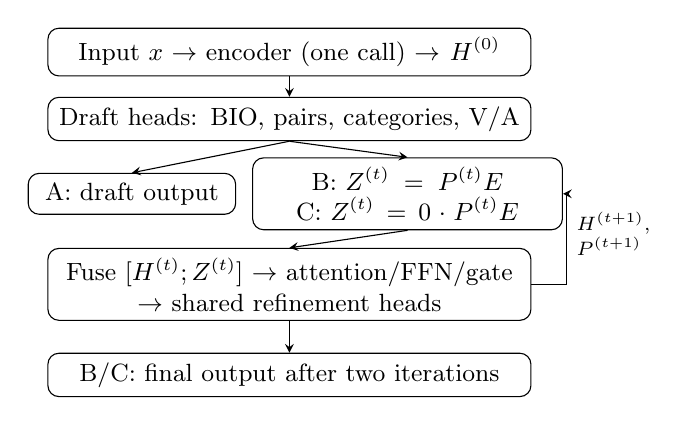
\begin{tikzpicture}[>=stealth, every node/.style={font=\small}, box/.style={draw,rounded corners,align=center,text width=5.9cm,minimum height=0.52cm}]
\node[box] (enc) at (0,0) {Input $x$ $\rightarrow$ encoder (one call) $\rightarrow H^{(0)}$};
\node[box] (draft) at (0,-0.85) {Draft heads: BIO, pairs, categories, V/A};
\node[box,text width=2.4cm] (a) at (-2,-1.8) {A: draft output};
\node[box,text width=3.7cm] (bc) at (1.5,-1.8) {B: $Z^{(t)}=P^{(t)}E$\\C: $Z^{(t)}=0\cdot P^{(t)}E$};
\node[box] (refine) at (0,-2.95) {Fuse $[H^{(t)};Z^{(t)}]$ $\rightarrow$ attention/FFN/gate\\$\rightarrow$ shared refinement heads};
\node[box] (out) at (0,-4.1) {B/C: final output after two iterations};
\draw[->] (enc)--(draft);
\draw[->] (draft.south)--(a.north);
\draw[->] (draft.south)--(bc.north);
\draw[->] (bc.south)--(refine.north);
\draw[->] (refine)--(out);
\draw[->] (refine.east)--++(0.45,0)|-node[pos=0.28,right,font=\scriptsize,align=left] {$H^{(t+1)}$,\\$P^{(t+1)}$} (bc.east);
\end{tikzpicture}
\caption{Active inference paths. B/C repeat the refinement block twice with shared weights. Only BIO predictions feed token refinement; the computed pair-fusion output is discarded. A bypasses refinement.}
\label{fig:feedback}
\end{figure}

Figure~\ref{fig:feedback} distinguishes the active paths in the three conditions.
Let $P^{(t)}$ denote the token-level BIO distribution and $E$ the learned label embedding matrix. The refinement path forms
\begin{equation}
 Z^{(t)}=P^{(t)}E,\qquad
 U^{(t)}=W_f[H^{(t)};Z^{(t)}]+b_f.
\end{equation}
Token fusion is followed by self-attention, feed-forward processing, and gated feature combination. Refined states are passed to the second-stage prediction heads. Two recurrent refinement calls reuse the refinement module and second-stage heads; the encoder is evaluated once. Only the BIO embedding is used as prediction feedback into the token path. Category and affect predictions are not consumed through an active pair-feedback path.

We compare three conditions. \textbf{A} is the single-stage extractor without refinement. \textbf{B} uses the implemented BIO-feedback network with two refinement calls. \textbf{C} uses the same network and calls as B, computes $Z^{(t)}$, and then replaces it by $0\cdot Z^{(t)}$ before token fusion at each call. B and C have identical allocated parameters and initial weights. However, zeroing blocks the task gradient through both $E$ and $P^{(t)}$ on this path; the corresponding input columns of $W_f$ also receive zero data gradient. In particular, C's draft BIO head receives no task gradient through feedback. This statement concerns loss gradients, not possible optimizer weight decay or EMA updates. B--C therefore measures the joint intervention on forward content and its learning path under this training recipe, rather than a content-only effect at identical effective capacity.

\subsection{Assignment and Training Objective}
Candidate pairs are aligned with gold quads by Hungarian assignment. For a gold quad $g$ and candidate $p$, the cost is
\begin{align}
 C(g,p)={}&2(2-\mathrm{IoU}_a-\mathrm{IoU}_o)\nonumber\\
 &-\log p_e(e_g)-\log p_c(c_g)\nonumber\\
 &+\frac{0.5}{8}(|V_p-V_g|+|A_p-A_g|).
\end{align}
Here the two classification terms refer to entity and attribute probabilities. Pair-validity loss is not a term in the assignment cost. Assignment uses normalized L1 affect distance; the regression training objective uses Huber loss. The fixed total objective is
\begin{align}
\mathcal L={}&2\mathcal L_{\rm BIO}+\mathcal L_{\rm pair}
 +\mathcal L_{\rm entity}+\mathcal L_{\rm attribute}\nonumber\\
 &+\mathcal L_{\rm VA}+0.5\mathcal L_{\rm consistency},
\end{align}
where the V/A components of $\mathcal L_{\rm VA}$ have weights 1 and 2. For B/C, consistency is the scalar BIO-loss margin penalty
\begin{equation}
\mathcal L_{\rm consistency}=\max(0,\mathcal L_{\rm BIO}^{\rm final}
-\operatorname{stopgrad}(\mathcal L_{\rm BIO}^{\rm draft})+0.1).
\end{equation}
The final BIO, pair, entity, and attribute cross-entropies use label smoothing of 0.1. The detached draft BIO loss in the margin term is unsmoothed, so the two scalar BIO losses are not identically defined. This term is an implementation-specific training penalty, not a guarantee that refinement improves predictions. It does not enforce pair, category, or V/A distribution agreement. A omits this term. All conditions use the same fixed objective weights for their shared components.

For B/C, the direct BIO cross-entropy supervises only the final output: there is no separate draft BIO loss or first-refinement loss in the objective. The draft loss enters solely as the detached margin reference. B's draft BIO head can learn indirectly through the differentiable feedback path; C cuts that path. The shared second-stage head receives direct supervision at its final invocation in both conditions. The detached reference can still affect whether the margin penalty is active, so the absence of a gradient through the reference does not make it numerically irrelevant. Five softmax coordinates alone do not establish useful BIO semantics at intermediate stages; we examine their decoded labels in the post-review diagnostics.

\section{Experimental Setup}
\subsection{Data and Scope}
\begin{table}[t]
\centering\small
\caption{Dataset sizes after removing training texts identical to development or unlabelled test texts.}\label{tab:data}
\begin{tabular}{lrrr}
\toprule
Dataset & Train & Dev & Test \\
\midrule
English restaurant & 2284 & 200 & 1000 \\
English laptop & 4075 & 200 & 1000 \\
Japanese hotel & 1597 & 200 & 800 \\
Russian restaurant & 1240 & 48 & 630 \\
Tatar restaurant & 1240 & 48 & 630 \\
Ukrainian restaurant & 1239 & 48 & 630 \\
Chinese restaurant & 6050 & 300 & 1000 \\
Chinese laptop & 3490 & 300 & 1000 \\
\bottomrule
\end{tabular}
\end{table}

We use eight Track~A language--domain datasets (Table~\ref{tab:data}). Gold-only training texts matching development or unlabelled test texts are removed using NFKC normalization, case folding, and whitespace normalization. Remaining row order and within-training multiplicity are retained. This is an exact-text check, not an audit of semantic overlap. Test labels are not used for this filtering.

The core matrix is three restaurant datasets $\times$ A/B/C $\times$ seeds 42, 123, and 456, giving 27 runs. The five-domain extension evaluates A with the same three seeds, adding 15 runs. Each run starts from the same pretrained encoder snapshot rather than a task-finetuned transfer checkpoint. There is no synthetic augmentation, distillation, or dataset-specific encoder search in this experiment. The earlier heterogeneous system configurations are not pooled into these controlled tables.

\subsection{Training and Selection}
All 42 runs use \path{microsoft/mdeberta-v3-base}, pinned to revision \texttt{a0484667b223} (full hash retained in the experiment manifest), with a fast tokenizer and maximum length 256. We use float32, batch size 8, no gradient accumulation, and 30 epochs without early stopping. Optimization uses AdamW with linear warmup followed by linear learning-rate decay. Encoder and head learning rates are $1.5\times10^{-5}$ and $7.5\times10^{-5}$; weight decay is 0.01, warmup ratio 0.1, dropout 0.1, and gradient clipping threshold 1.0. FGM uses $\epsilon=0.1$ after the initial warmup; EMA decay is 0.999. CRF decoding, uncertainty-based loss weighting, and category embedding options are disabled.

For each core seed, shared A/B/C initial tensors and all B/C tensors are checked by byte fingerprints. An independent epoch sampler fixes minibatch order across paired conditions; actual update counts and order hashes are audited. Different architectures need not consume identical dropout random-number sequences. Selection uses the highest local development cF1 over 30 epochs; exact ties retain the earliest epoch. We restore that checkpoint's EMA parameters, without averaging checkpoints or reselecting under the official scorer.

Official development scores are recomputed for all runs. Local and official scorers differ in string normalization and handling of categorical keys, so their values are not assumed interchangeable. Inference requires the valid-pair class to win the argmax and its probability to meet a fixed threshold of 0.3. Since validity is binary, the argmax already imposes an effective boundary of approximately 0.5; 0.3 is not the operative acceptance boundary. We use no top-$k$ span expansion and no dual-layer decoding. The secondary ensemble keeps an exact categorical triple when at least two of the three fixed seeds predict it, then averages the contributing V/A values. No seed or vote threshold is selected on test data.

\subsection{Companion Materials and Versioning}
The companion \texttt{paper\_icsai\_v3\_source.zip} includes the supplement, code, configurations, and audit records. Start with \path{docs/ICSAI_REPRODUCIBILITY_V3.md} for exact design, implementation, scorer, and artifact identities. New diagnostics are recorded separately as post-review analyses. The archive supports table rebuilding; full inference replay additionally requires the identified local checkpoints, original quad predictions, and data from the official DimABSA repository~\cite{dimabsa2026,overview2026}, which are not bundled.

\subsection{Evaluation Integrity and Statistics}
Historical test results had already been exposed before the present experimental design. We therefore describe these runs as \emph{post-competition, post-test-exposure fixed-protocol supplementary evaluations}. Model files, inference settings, and input identities are frozen before new test inference; all prediction hashes are frozen before their scores are computed. This procedure limits further selection within the present experiment but cannot reverse earlier test exposure.

We retain every seed result in the experiment records and report cF1 in the main tables as its three-seed mean and sample standard deviation. On the three core datasets, B--A and B--C form a family of six contrasts. We perform 10,000 paired sentence bootstrap resamples with seed 20260907, sharing each resample across all arms and training seeds and then averaging per-seed score differences. Percentile 95\% intervals are unadjusted. A two-sided centered bootstrap $p$ value is computed as
\begin{equation}
 p=\frac{1+\sum_{b=1}^{10000}\mathbf{1}\{|\Delta_b^*-\widehat\Delta|\geq|\widehat\Delta|\}}{10001},
\end{equation}
and Holm correction is applied across the six test contrasts. This uncertainty is conditional on the three trained seeds; it does not estimate variability of the full training or model-development procedure. Eight-domain macro means are equal-domain descriptive averages, without an additional significance claim.

\section{Results and Discussion}
\subsection{Uniform Eight-Dataset Evaluation}
\begin{table}[t]
\centering\small
\caption{Official test cF1 for A: three-seed mean and sample SD; fixed vote-2 ensemble. Macro values are descriptive.}\label{tab:eight}
\begin{tabular}{lcc}
\toprule
Dataset & Single model & Ensemble \\
\midrule
English laptop & $0.2460\pm0.0117$ & 0.2667 \\
English restaurant & $0.5321\pm0.0028$ & 0.5575 \\
Japanese hotel & $0.2362\pm0.0025$ & 0.2514 \\
Russian restaurant & $0.3997\pm0.0124$ & 0.4326 \\
Tatar restaurant & $0.3332\pm0.0171$ & 0.3682 \\
Ukrainian restaurant & $0.3713\pm0.0377$ & 0.4252 \\
Chinese laptop & $0.3492\pm0.0056$ & 0.3794 \\
Chinese restaurant & $0.3833\pm0.0050$ & 0.4091 \\
Equal-domain mean & 0.3564 & 0.3862 \\
\bottomrule
\end{tabular}
\end{table}

Table~\ref{tab:eight} reports the eight-dataset A evaluation. The mean single-model cF1 is 0.3564; the fixed ensemble reaches 0.3862, a descriptive increase of 2.99 percentage points. The ensemble score exceeds the corresponding seed-mean single-model score on every dataset. This observation supports fixed voting as a useful option within the evaluated runs, but is not a comparison against the best seed selected with test information. It also entails three model evaluations, so the performance increase should not be presented as cost-free.

The uniform protocol obtains different absolute scores across datasets. English restaurant reaches 0.5321, whereas Japanese hotel and English laptop reach 0.2362 and 0.2460. These differences cannot be attributed solely to language or interpreted as a ranking of language difficulty: domain, annotation structure, data size, tokenization, and extraction difficulty also vary. Ukrainian restaurant exhibits a seed SD of 0.0377, reinforcing the importance of reporting multiple runs rather than a single favorable checkpoint.

\subsection{Does Refinement Benefit from BIO Feedback?}
\begin{table}[t]
\centering\small\setlength{\tabcolsep}{3pt}
\caption{Core restaurant test cF1 (mean $\pm$ sample SD over three seeds).}\label{tab:ablation}
\begin{tabular}{lccc}
\toprule
Language & A & B & C \\
\midrule
English & $0.5321\pm0.0028$ & $0.5380\pm0.0033$ & $0.5324\pm0.0156$ \\
Chinese & $0.3833\pm0.0050$ & $0.3737\pm0.0037$ & $0.3715\pm0.0092$ \\
Tatar & $0.3332\pm0.0171$ & $0.3169\pm0.0228$ & $0.3285\pm0.0067$ \\
\bottomrule
\end{tabular}
\end{table}

\begin{table}[t]
\centering\small
\caption{Paired test contrasts in cF1 percentage points. Percentile intervals are unadjusted; $p$ values use Holm correction over all six contrasts.}\label{tab:contrasts}
\begin{tabular}{llrrr}
\toprule
Language & Contrast & $\Delta$ & 95\% CI & $p_{\rm Holm}$ \\
\midrule
English & B-A & +0.59 & $[-0.12,+1.29]$ & 0.2014 \\
English & B-C & +0.56 & $[-0.01,+1.13]$ & 0.1659 \\
Chinese & B-A & -0.96 & $[-1.71,-0.21]$ & 0.0730 \\
Chinese & B-C & +0.22 & $[-0.35,+0.80]$ & 0.4418 \\
Tatar & B-A & -1.62 & $[-2.72,-0.46]$ & 0.0222 \\
Tatar & B-C & -1.16 & $[-2.11,-0.19]$ & 0.0816 \\
\bottomrule
\end{tabular}
\end{table}

The core comparison is in Tables~\ref{tab:ablation} and~\ref{tab:contrasts}. B exceeds A by 0.59 percentage points on English restaurant, but falls below it by 0.96 points on Chinese and 1.62 points on Tatar. After Holm correction, only the Tatar B--A contrast reaches the 0.05 threshold ($p=0.0222$), and its direction is negative. The result therefore provides no corrected evidence of a positive refinement benefit across the core datasets. B--A changes the architecture and the consistency penalty together, so this contrast alone cannot attribute an effect specifically to BIO content.

B--C targets the implemented BIO feedback path more directly than B--A, while jointly changing its forward content and task-gradient route. Its differences are +0.56, +0.22, and -1.16 points for English, Chinese, and Tatar, respectively, and none passes Holm correction. Failure to reject a zero difference does not establish equivalence. In particular, the experiment neither proves that prediction feedback is intrinsically ineffective nor identifies why Tatar deteriorates. It shows that this implementation and training recipe do not deliver a robust positive effect on the evaluated datasets.

The test findings also qualify development-set impressions. Official English development cF1 favored B over A by about 1.80 points, whereas the corresponding test difference is smaller and uncertain. The checkpoints remain those chosen by the original local development rule. We do not tune the refinement mechanism after inspecting these outcomes or expand the core comparison selectively to seek a favorable language.

The supplement reports all paired seed differences. For example, Tatar B--A differences are -3.52, -0.90, and -0.45 percentage points for seeds 42, 123, and 456. Their common negative sign and unequal magnitudes distinguish the observed seed behavior from the sentence-bootstrap uncertainty conditional on these fixed models.

\subsection{Intermediate BIO Diagnostics}
\begin{table}[t]
\centering\small
\setlength{\tabcolsep}{3pt}
\caption{Post-review development typed token-span F1, averaged over three fixed seeds. A has only a draft output. These are diagnostics of the existing BIO projection, not official quad scores.}\label{tab:stages}
\begin{tabular}{llrrr}
\toprule
Language & Arm & Draft & Refine 1 & Final \\
\midrule
English & A & 0.855 & -- & -- \\
English & B & 0.102 & 0.830 & 0.856 \\
English & C & 0.046 & 0.831 & 0.852 \\
Chinese & A & 0.736 & -- & -- \\
Chinese & B & 0.082 & 0.723 & 0.729 \\
Chinese & C & 0.011 & 0.737 & 0.737 \\
Tatar & A & 0.708 & -- & -- \\
Tatar & B & 0.050 & 0.683 & 0.707 \\
Tatar & C & 0.006 & 0.696 & 0.706 \\
\bottomrule
\end{tabular}
\end{table}

After review, we inspect all 27 fixed core checkpoints on their original development splits using forward hooks on the unmodified span heads. Every final quad output exactly reproduces the archived development prediction. No training, checkpoint reselection, or threshold adjustment is performed. We compute exact-tag non-O BIO micro F1 and exact typed token-span F1, scoring attended positions including CLS/SEP and excluding padding. Gold spans are decoded from the existing five-way BIO projection; this diagnostic does not recover annotations lost through overlapping labels or truncation. The supplement reports BIO accuracy, non-O F1, span F1, sample SDs, and per-run records.

Table~\ref{tab:stages} shows that B's mean draft span F1 is 0.102, 0.082, and 0.050 for English, Chinese, and Tatar, compared with A's directly supervised output at 0.855, 0.736, and 0.708. B's first-refinement scores rise to 0.830, 0.723, and 0.683, and its final scores are 0.856, 0.729, and 0.707. C also develops substantially stronger later outputs despite removing feedback. Thus B's initial channel cannot be characterized as an accurate decoded boundary estimate under the intended labels. Low decoded F1 does not establish that its soft representation is uninformative; the first-refinement head also shares weights with the directly supervised final head. These observations qualify the interpretation of prediction feedback but do not identify the cause of the Tatar test decrease or predict the effect of adding direct draft supervision.

\subsection{Extraction and Affect Diagnostics}
\begin{table}[t]
\centering\small
\caption{A model diagnostics, averaged across seeds. Coverage is the proportion of gold quads with exactly one categorical match; V/A MAE is conditional on these matches.}\label{tab:diag}
\begin{tabular}{lrrrr}
\toprule
Dataset & F1 & Cov. & V MAE & A MAE \\
\midrule
English laptop & 0.265 & 0.257 & 0.508 & 0.583 \\
English restaurant & 0.578 & 0.581 & 0.556 & 0.661 \\
Japanese hotel & 0.247 & 0.258 & 0.284 & 0.342 \\
Russian restaurant & 0.452 & 0.465 & 0.722 & 1.034 \\
Tatar restaurant & 0.378 & 0.384 & 0.761 & 1.046 \\
Ukrainian restaurant & 0.416 & 0.439 & 0.670 & 0.968 \\
Chinese laptop & 0.365 & 0.367 & 0.282 & 0.344 \\
Chinese restaurant & 0.408 & 0.429 & 0.405 & 0.499 \\
\bottomrule
\end{tabular}
\end{table}

Table~\ref{tab:diag} separates categorical extraction F1 from conditional affect error for A. Coverage is the fraction of gold quads with exactly one categorical match, and V/A MAE is computed only on those matches. Low conditional MAE cannot compensate for missing categorical structures, nor does it characterize affect error on unmatched quads. These diagnostics help interpret cF1 without assigning an unsupported single cause to cross-dataset differences. All 56 test prediction files from the core and extension studies were cross-checked against the pinned official evaluator; their prediction locks were verified again when generating the manuscript tables.

\subsection{Illustrative Cases and Their Selection}
\begin{table*}[t]
\centering\small
\caption{Deterministically selected English restaurant dev examples (seed 42). IDs omit the common \texttt{rest26\_asqp\_dev\_} prefix. Cases illustrate outcomes, not their prevalence or cause. All categorical comparisons lowercase strings.}
\label{tab:cases}
\begin{tabular}{lp{5.1cm}p{10.0cm}}
\toprule
ID & Input sentence & Observed outputs \\
\midrule
2 & Customer service was fantastic and food was awesome & A recovers both gold categorical triples. For Customer service/fantastic, gold V/A is 7.33/7.33 and A predicts 8.26/8.33. B splits Customer service into two aspect spans; C preserves the gold categorical structure. \\
29 & Service is attentive and they got my picky order straight & Gold contains one Service/attentive triple. A predicts that triple plus an extra NULL/attentive triple; B and C predict only the gold categorical triple. Their V/A values still differ from the gold annotation. \\
23 & Mac 'n Cheese was good and a little spicy & Gold associates the aspect with both good and a little spicy. A recovers both categorical triples; B and C retain only good. All categories in this example are FOOD\#QUALITY. \\
\bottomrule
\end{tabular}
\end{table*}

We inspect existing English restaurant development predictions for seed 42 using an explicit deterministic rule. In original row order, we take the first unused example for each of four ordered strata: A recovers the complete nonempty categorical set; A fails and B succeeds; A succeeds and B fails; and A misses a gold triple containing a NULL aspect or opinion. Success requires identical lowercased categorical multisets without duplicate predicted keys. These rules select IDs 2, 29, and 23; the fourth stratum has no eligible example and is not replaced. Full predictions, source hashes, and eligibility counts are retained in the case audit. The rule was fixed before this case extraction, after prior exposure to the predictions, and is not a blind sampling protocol.

Table~\ref{tab:cases} illustrates why categorical success does not imply perfect cF1: A's correct service extraction in ID~2 still has affect error. In ID~29, B removes an extra triple present in A; C does so as well, so this example does not uniquely support BIO feedback. ID~23 illustrates the opposite outcome, with both refinement conditions omitting a gold opinion. These outcome-stratified examples are selected for illustration, not to estimate error prevalence or explain the Tatar test decrease. They concern one English development seed and cannot replace the paired test analysis.

\subsection{Implicit-Element Coverage}
All three core test datasets contain no NULL gold quads. Japanese hotel, in the extension, contains 152 of 800 sentences with at least one NULL element, and 175 implicit quads among 1,443 total gold quads. A's mean cF1 is 0.2225 on those 152 sentences and 0.2402 on the 648 explicit-only sentences, retaining every quad in each selected sentence. A separate quad partition, assigning gold and predicted quads by their own NULL status across all 800 sentences, gives 0.1914 for implicit and 0.2416 for explicit quads. The fixed ensemble and per-seed values appear in the supplement. These post-review descriptions demonstrate nonzero implicit extraction in the implemented system. They neither attribute the Japanese score gap solely to NULL handling nor estimate the benefit of adding another anchor. No Japanese test gold quad has both elements NULL, although the single-layer anchor collision remains a structural limitation for sentences requiring both types at position 0.

\subsection{Repeated Inference Cost}
\begin{table}[t]
\centering\small\setlength{\tabcolsep}{3pt}
\caption{Repeated cost on 64 fixed English development sentences. Wall time includes decoding and, for ensembles, voting; memory is peak allocated GPU memory. Single-model SD combines three seeds and five repeats per seed.}\label{tab:cost}
\begin{tabular}{llrrr}
\toprule
Arm & Mode & Seconds $\pm$ SD & Rows/s & GiB \\
\midrule
A & Single & $0.232\pm0.002$ & 276.3 & 1.32 \\
A & Ensemble & $0.699\pm0.002$ & 91.5 & 3.43 \\
B & Single & $0.358\pm0.013$ & 179.0 & 1.38 \\
B & Ensemble & $1.073\pm0.006$ & 59.7 & 3.60 \\
C & Single & $0.371\pm0.017$ & 172.4 & 1.38 \\
C & Ensemble & $1.111\pm0.004$ & 57.6 & 3.60 \\
\bottomrule
\end{tabular}
\end{table}

We benchmark the first 64 English restaurant development sentences in their existing order, stripping their labels. The workload is fixed before measurement and is not selected by model accuracy. All runs use the same RTX 4090, float32, batch size 8, maximum length 256, and pretokenized CPU batches. After one complete warmup pass, each seed model is measured five times while it alone resides on the GPU. For each arm, the fixed three-seed ensemble is measured five times with all three models resident and evaluated sequentially. CUDA synchronization brackets each inference pass; timing includes host-to-device transfers and decoding, plus CPU voting for ensembles. Tokenization and loading are excluded; CPU loading durations are recorded separately after checkpoint hash verification and are not cold-cache measurements.

Table~\ref{tab:cost} reports mean wall time, sample SD, throughput, and peak allocated GPU memory. Single-model variation combines three seeds and five repeats per seed; ensemble variation covers five repeats. Identical outputs across repeats are checked. B takes 1.54 times A's mean single-model inference time on this workload. The ensemble rows measure a specified residency policy, not every possible deployment strategy. Arms were measured in fixed A/B/C order rather than counterbalanced order, so small differences may include temporal effects. These measurements establish a local cost comparison for a short fixed English workload, not an all-language latency guarantee. They should be interpreted alongside the mixed feedback accuracy findings, rather than used alone to choose a universally preferable system.

\subsection{Scope and Limitations}
In the core configuration, A allocates 282,528,790 parameters and B/C each allocate 297,125,356, an increase of approximately 5.17\%. Table~\ref{tab:cost} complements parameter counts with repeated measurements under one explicit inference setup. Input length, language, hardware, concurrency, and model-residency choices may change the deployment trade-off.

The gold-only study does not establish the fidelity or utility of synthetic augmentation from the earlier system. Such claims require a separate label-preservation audit and are not made here. Fast-tokenizer offset reconstruction is another boundary: SentencePiece byte fallback is not reproduced completely by the fast tokenizer, and limited tokenizer checks do not rule out rare-character effects. Finally, the feedback intervention covers three restaurant datasets and a fixed base encoder. It does not establish effects for all eight datasets, larger encoders, alternative feedback designs, or the full history of hyperparameter selection.

\section{Conclusion}
A fixed evaluation of LEADER-DimASQP distinguishes single-stage extraction, BIO-feedback refinement, and refinement with zeroed feedback. Across three core datasets, no positive contrast survives correction; Tatar shows a corrected decrease relative to the single-stage model. Development stage diagnostics reveal weak decoded draft boundaries despite stronger later outputs, qualifying a semantic interpretation of the initial feedback channel. B--C intervenes on both forward content and its gradient path. A uniform single-stage protocol provides an eight-dataset reference, with a descriptive improvement from fixed three-seed voting. Repeated measurements on a fixed English workload show additional inference cost for refinement and three-seed voting. These results remain supplementary evaluations after prior test exposure.

\begin{thebibliography}{14}
\bibitem{cai2021acos} H. Cai, R. Xia, and J. Yu, ``Aspect-category-opinion-sentiment quadruple extraction with implicit aspects and opinions,'' in \emph{Proc. ACL-IJCNLP}, 2021, pp. 340--350, doi: 10.18653/v1/2021.acl-long.29.
\bibitem{zhang2021asqp} W. Zhang, Y. Deng, X. Li, Y. Yuan, L. Bing, and W. Lam, ``Aspect sentiment quad prediction as paraphrase generation,'' in \emph{Proc. EMNLP}, 2021, pp. 9209--9219, doi: 10.18653/v1/2021.emnlp-main.726.
\bibitem{dimabsa2026} L.-H. Lee et al., ``DimABSA: Building multilingual and multidomain datasets for dimensional aspect-based sentiment analysis,'' arXiv:2601.23022v3, 2026. [Online]. Available: \url{https://arxiv.org/abs/2601.23022}
\bibitem{overview2026} L.-C. Yu et al., ``SemEval-2026 Task 3: Dimensional aspect-based sentiment analysis (DimABSA),'' arXiv:2604.07066, 2026. [Online]. Available: \url{https://arxiv.org/abs/2604.07066}
\bibitem{qin2026leader} H. Qin, Y. Suzuki, F. Fukumoto, and R. Zhou, ``LEADER-DimASQP: Language-specific encoder and data-aware ensemble refinement for dimensional ASQP,'' earlier system manuscript, 2026. Archived source: \path{docs/paper_iconip_current.tex} in the companion archive; version identified in the supplement.
\bibitem{zhou2023one} J. Zhou, H. Yang, Y. He, H. Mou, and J. Yang, ``A unified one-step solution for aspect sentiment quad prediction,'' in \emph{Findings of ACL}, 2023, pp. 12249--12265, doi: 10.18653/v1/2023.findings-acl.777.
\bibitem{kim2024scrap} J. Kim et al., ``Self-consistent reasoning-based aspect-sentiment quad prediction with extract-then-assign strategy,'' in \emph{Findings of ACL}, 2024, pp. 7295--7303, doi: 10.18653/v1/2024.findings-acl.435.
\bibitem{gazetas2026ails} S. Gazetas, G. Filandrianos, M. Lymperaiou, P. Tzouveli, A. Voulodimos, and G. Stamou, ``AILS-NTUA at SemEval-2026 Task 3: Efficient dimensional aspect-based sentiment analysis,'' arXiv:2603.04933, 2026.
\bibitem{devink2026quad} A. J. W. de Vink, F. K. Ventirozos, N. Amat-Lefort, and L. Han, ``QuadAI at SemEval-2026 Task 3: Ensemble learning of hybrid RoBERTa and LLMs for dimensional aspect-based sentiment analysis,'' arXiv:2603.07766, 2026.
\bibitem{hikal2026logsigma} B. Hikal, J. Becker, and B. Gipp, ``LogSigma at SemEval-2026 Task 3: Uncertainty-weighted multitask learning for dimensional aspect-based sentiment analysis,'' arXiv:2603.24896, 2026.
\bibitem{he2019imn} R. He, W. S. Lee, H. T. Ng, and D. Dahlmeier, ``An interactive multi-task learning network for end-to-end aspect-based sentiment analysis,'' in \emph{Proc. ACL}, 2019, pp. 504--515, doi: 10.18653/v1/P19-1048.
\bibitem{liang2021imktn} Y. Liang, F. Meng, J. Zhang, Y. Chen, J. Xu, and J. Zhou, ``An iterative multi-knowledge transfer network for aspect-based sentiment analysis,'' in \emph{Findings of EMNLP}, 2021, pp. 1768--1780, doi: 10.18653/v1/2021.findings-emnlp.152.
\bibitem{he2023deberta} P. He, J. Gao, and W. Chen, ``DeBERTaV3: Improving DeBERTa using ELECTRA-style pre-training with gradient-disentangled embedding sharing,'' in \emph{Proc. ICLR}, 2023.
\bibitem{kuhn1955hungarian} H. W. Kuhn, ``The Hungarian method for the assignment problem,'' \emph{Naval Research Logistics Quarterly}, vol. 2, nos. 1--2, pp. 83--97, 1955, doi: 10.1002/nav.3800020109.
\end{thebibliography}
\end{document}
